\section{実験方法}
提案システムの各シーケンスにおいて消費電力を求めるため,起動からネットワーク参加,起動からネットワーク参加・初回送信,定常時の送信,スリープとイベントごと消費電力を計測する必要がある.実験では,市販のArduino互換LoRaWANモジュール及び消費電力計を用いて,消費電力を計測した.実験環境は,下記の表に示す.実験機材は,LoRaWANの送信機に,Arduino Uno R3\ref{fig:Arduino_Spec},LoRaWAN Shield for Arduino\ref{fig:LoRaWAN_Spec},受信機にLoRaWAN Gateway\ref{fig:LoRaWAN_Gateway_Spec},消費電力測定にKotomi Premium\ref{fig:Kotomi_Spec}を用いた.LoRaWANは長距離伝送がユースケースであるため,LoRaWANのノードとGWノードを,高低差があり,約3.5kmの距離がある公立はこだて未来大学と自宅間に配置した.また計測結果を保存できる容量に限りがあるため,3試行を1セットとした.LoRaWANの設定内容を述べる.前述したLoRaWANのADR機能を適応し,スリープ時間は4秒とした.30秒間の計測を4セット12試行した.パケット到達率を算出するため,データ受信を確認する必要がある.本実測で利用したLoRaWANモジュールのプロバイダーは,MQTTブローカーが提供しているため,MQTTクライアント(Eclipse Mosquitto)を用いてデータを取得した.下記図\ref{fig:experiment}は,実験の様子である.

\begin{table}[]
    \caption{ARDUINO UNO REV3}\label{fig:Arduino_Spec}
    \centering
    \begin{tabular}{|c|c|}
    \hline
    動作電圧     & 5V   \\ \hline
    DC電流     & 50mA \\ \hline
    フラッシュメモリ & 32KB \\ \hline
    SRAM     & 2KB  \\ \hline
    EEPROM   & 1KB  \\ \hline
    \end{tabular}
\end{table}

\begin{table}[]
    \caption{LoRaWAN Shield for Arduino}\label{fig:LoRaWAN_Spec}
    \centering
    \begin{tabular}{|c|c|}
    \hline
    電源電圧 & DC2.2 $\sim$3.6V      \\ \hline
    周波数  & 920.6MHz $\sim$928MHz \\ \hline
    動作温度 & 0°C $\sim$40 °C       \\ \hline
    サイズ  & 68mm×53mm × 22.8mm    \\ \hline
    無線規格 & LoRaWAN 1.0.2         \\ \hline
    \end{tabular}
\end{table}

\begin{table}[]
    \caption{Kotomi Premium}\label{fig:Kotomi_Spec}
    \centering
    \begin{tabular}{|l|l|}
    \hline
    サイズ    & 77 x 35 x 13mm \\ \hline
    ディスプレイ & 1.44インチ        \\ \hline
    電圧精度   & 0.0001V        \\ \hline
    電流制度   & 0.0001A        \\ \hline
    電圧範囲   & 3.7~25V        \\ \hline
    電流範囲   & 0~5A           \\ \hline
    \end{tabular}
\end{table}

\begin{table}[]
    \caption{LoRaWAN Gateway}\label{fig:LoRaWAN_Gateway_Spec}
    \centering
    \begin{tabular}{|c|c|}
    \hline
    モデル名         & SW-GW01                       \\ \hline
    チャンネル数       & 最大8ch                         \\ \hline
    Wireless LAN & 802.11 b/g/n 2.4G             \\ \hline
    送信出力         & 20mW (最大13 dBm)               \\ \hline
    受信感度         & Down to -142 dBm              \\ \hline
    動作温度         & -10ºC $\sim$55ºC              \\ \hline
    電源電圧         & DC 5V / 2A(ミニUSBポート経由)        \\ \hline
    インターフェース     & Ethernet x 1ポート, 3/4G USBドングル \\ \hline
    サイズ          & L:116 x W:91 x H:27 mm        \\ \hline
    重量           & 160g                          \\ \hline
    \end{tabular}
\end{table}

\begin{table}[]
    \caption{実測に用いた電源}\label{fig:LoRaWAN_Battery}
    \centering
    \begin{tabular}{|c|c|}
    \hline
    サイズ     & 72 x 70 x 31 (mm) \\ \hline
    重量      & 189g              \\ \hline
    バッテリー容量 & 5000mAh           \\ \hline
    入力      & 5V=2A             \\ \hline
    出力      & 5V=3A             \\ \hline
    \end{tabular}
\end{table}

\begin{figure}[]
    \begin{center}
    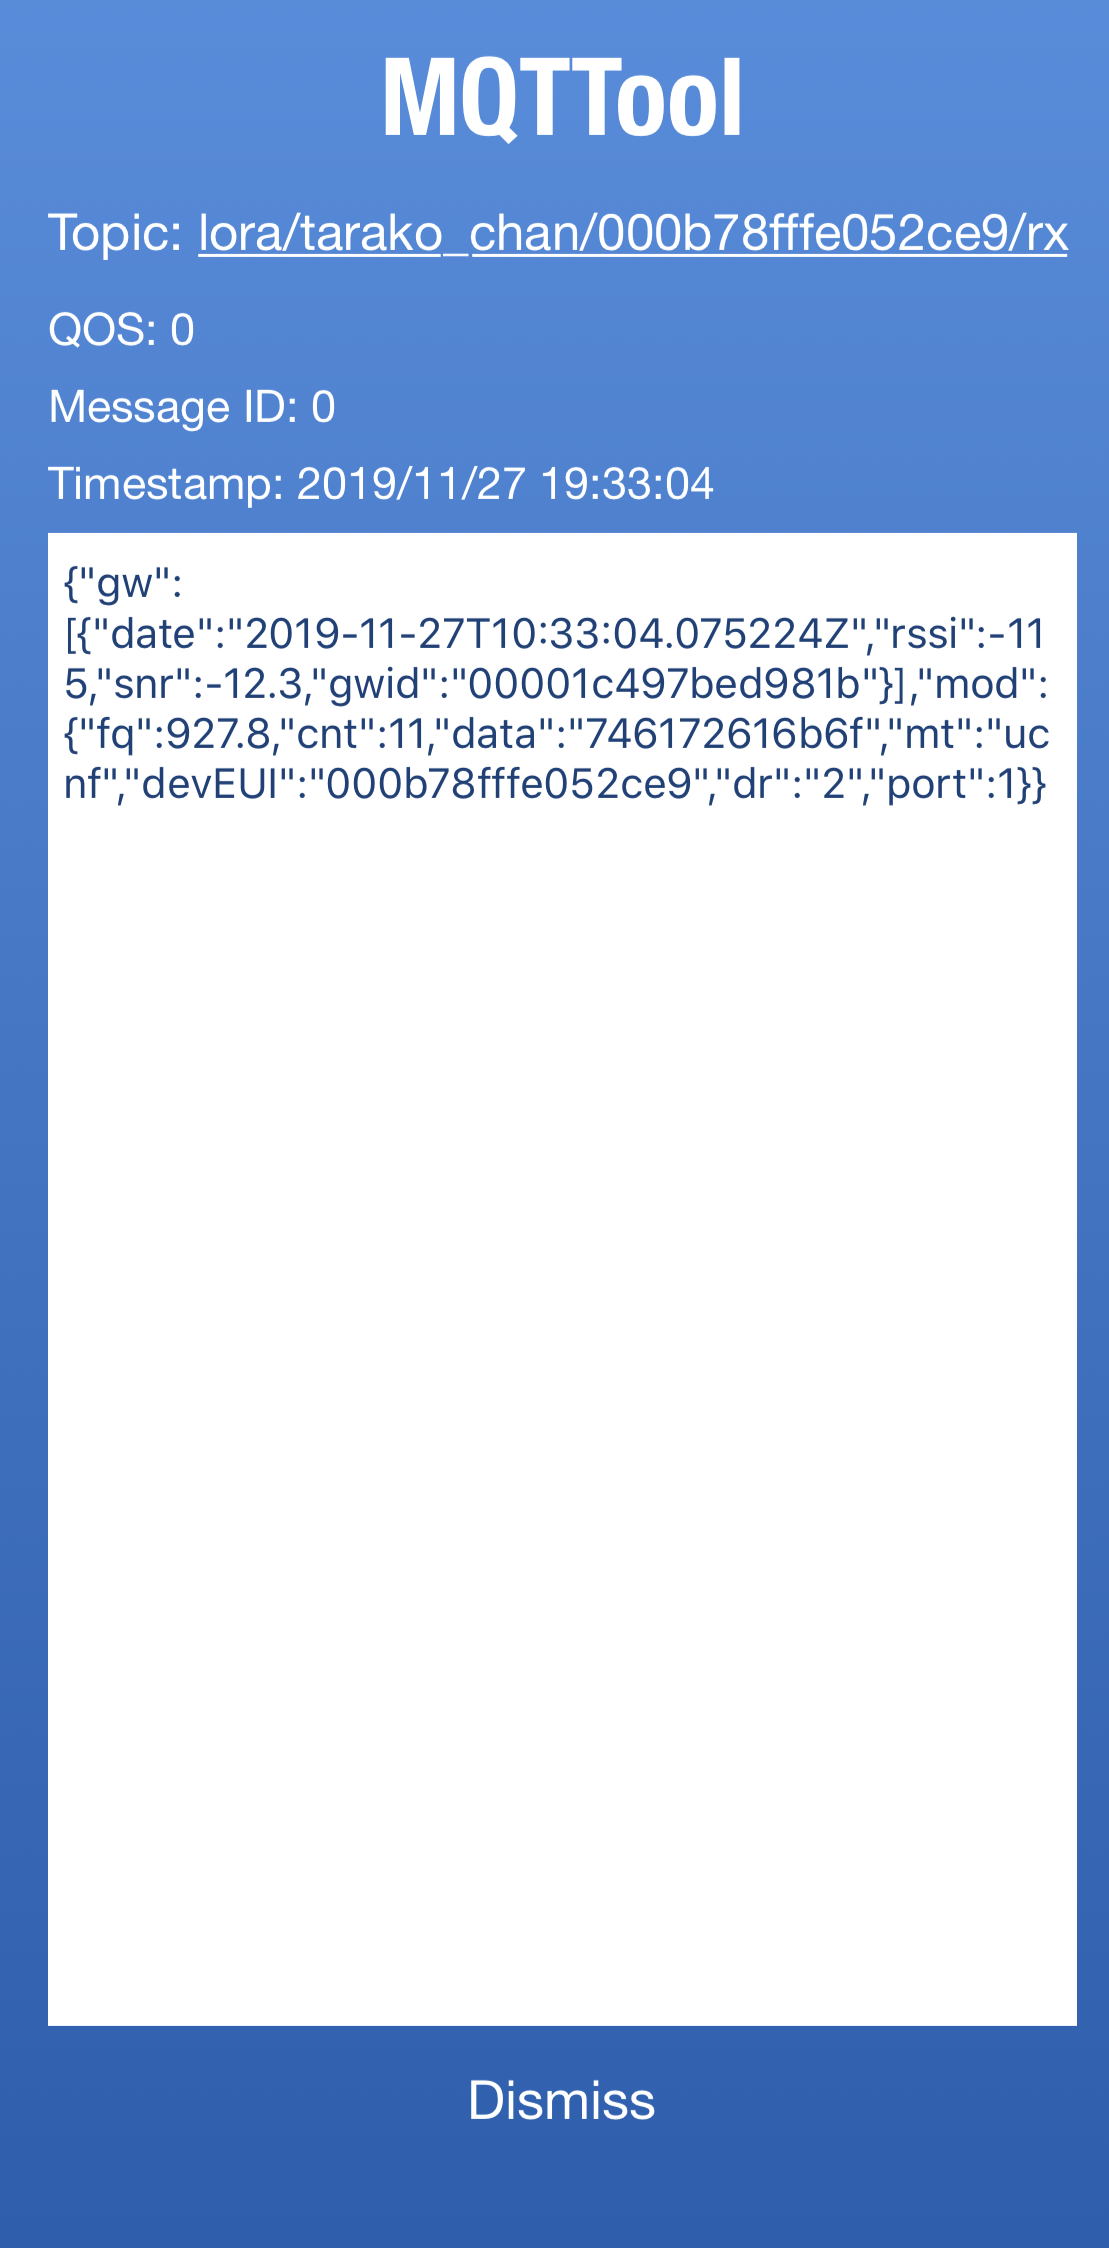
\includegraphics[width=5cm]{figures/mqtt.PNG}
    \caption{MQTT Client}
    \label{fig:mqtt}
    \end{center}
\end{figure}

\begin{figure}[]
    \begin{center}
    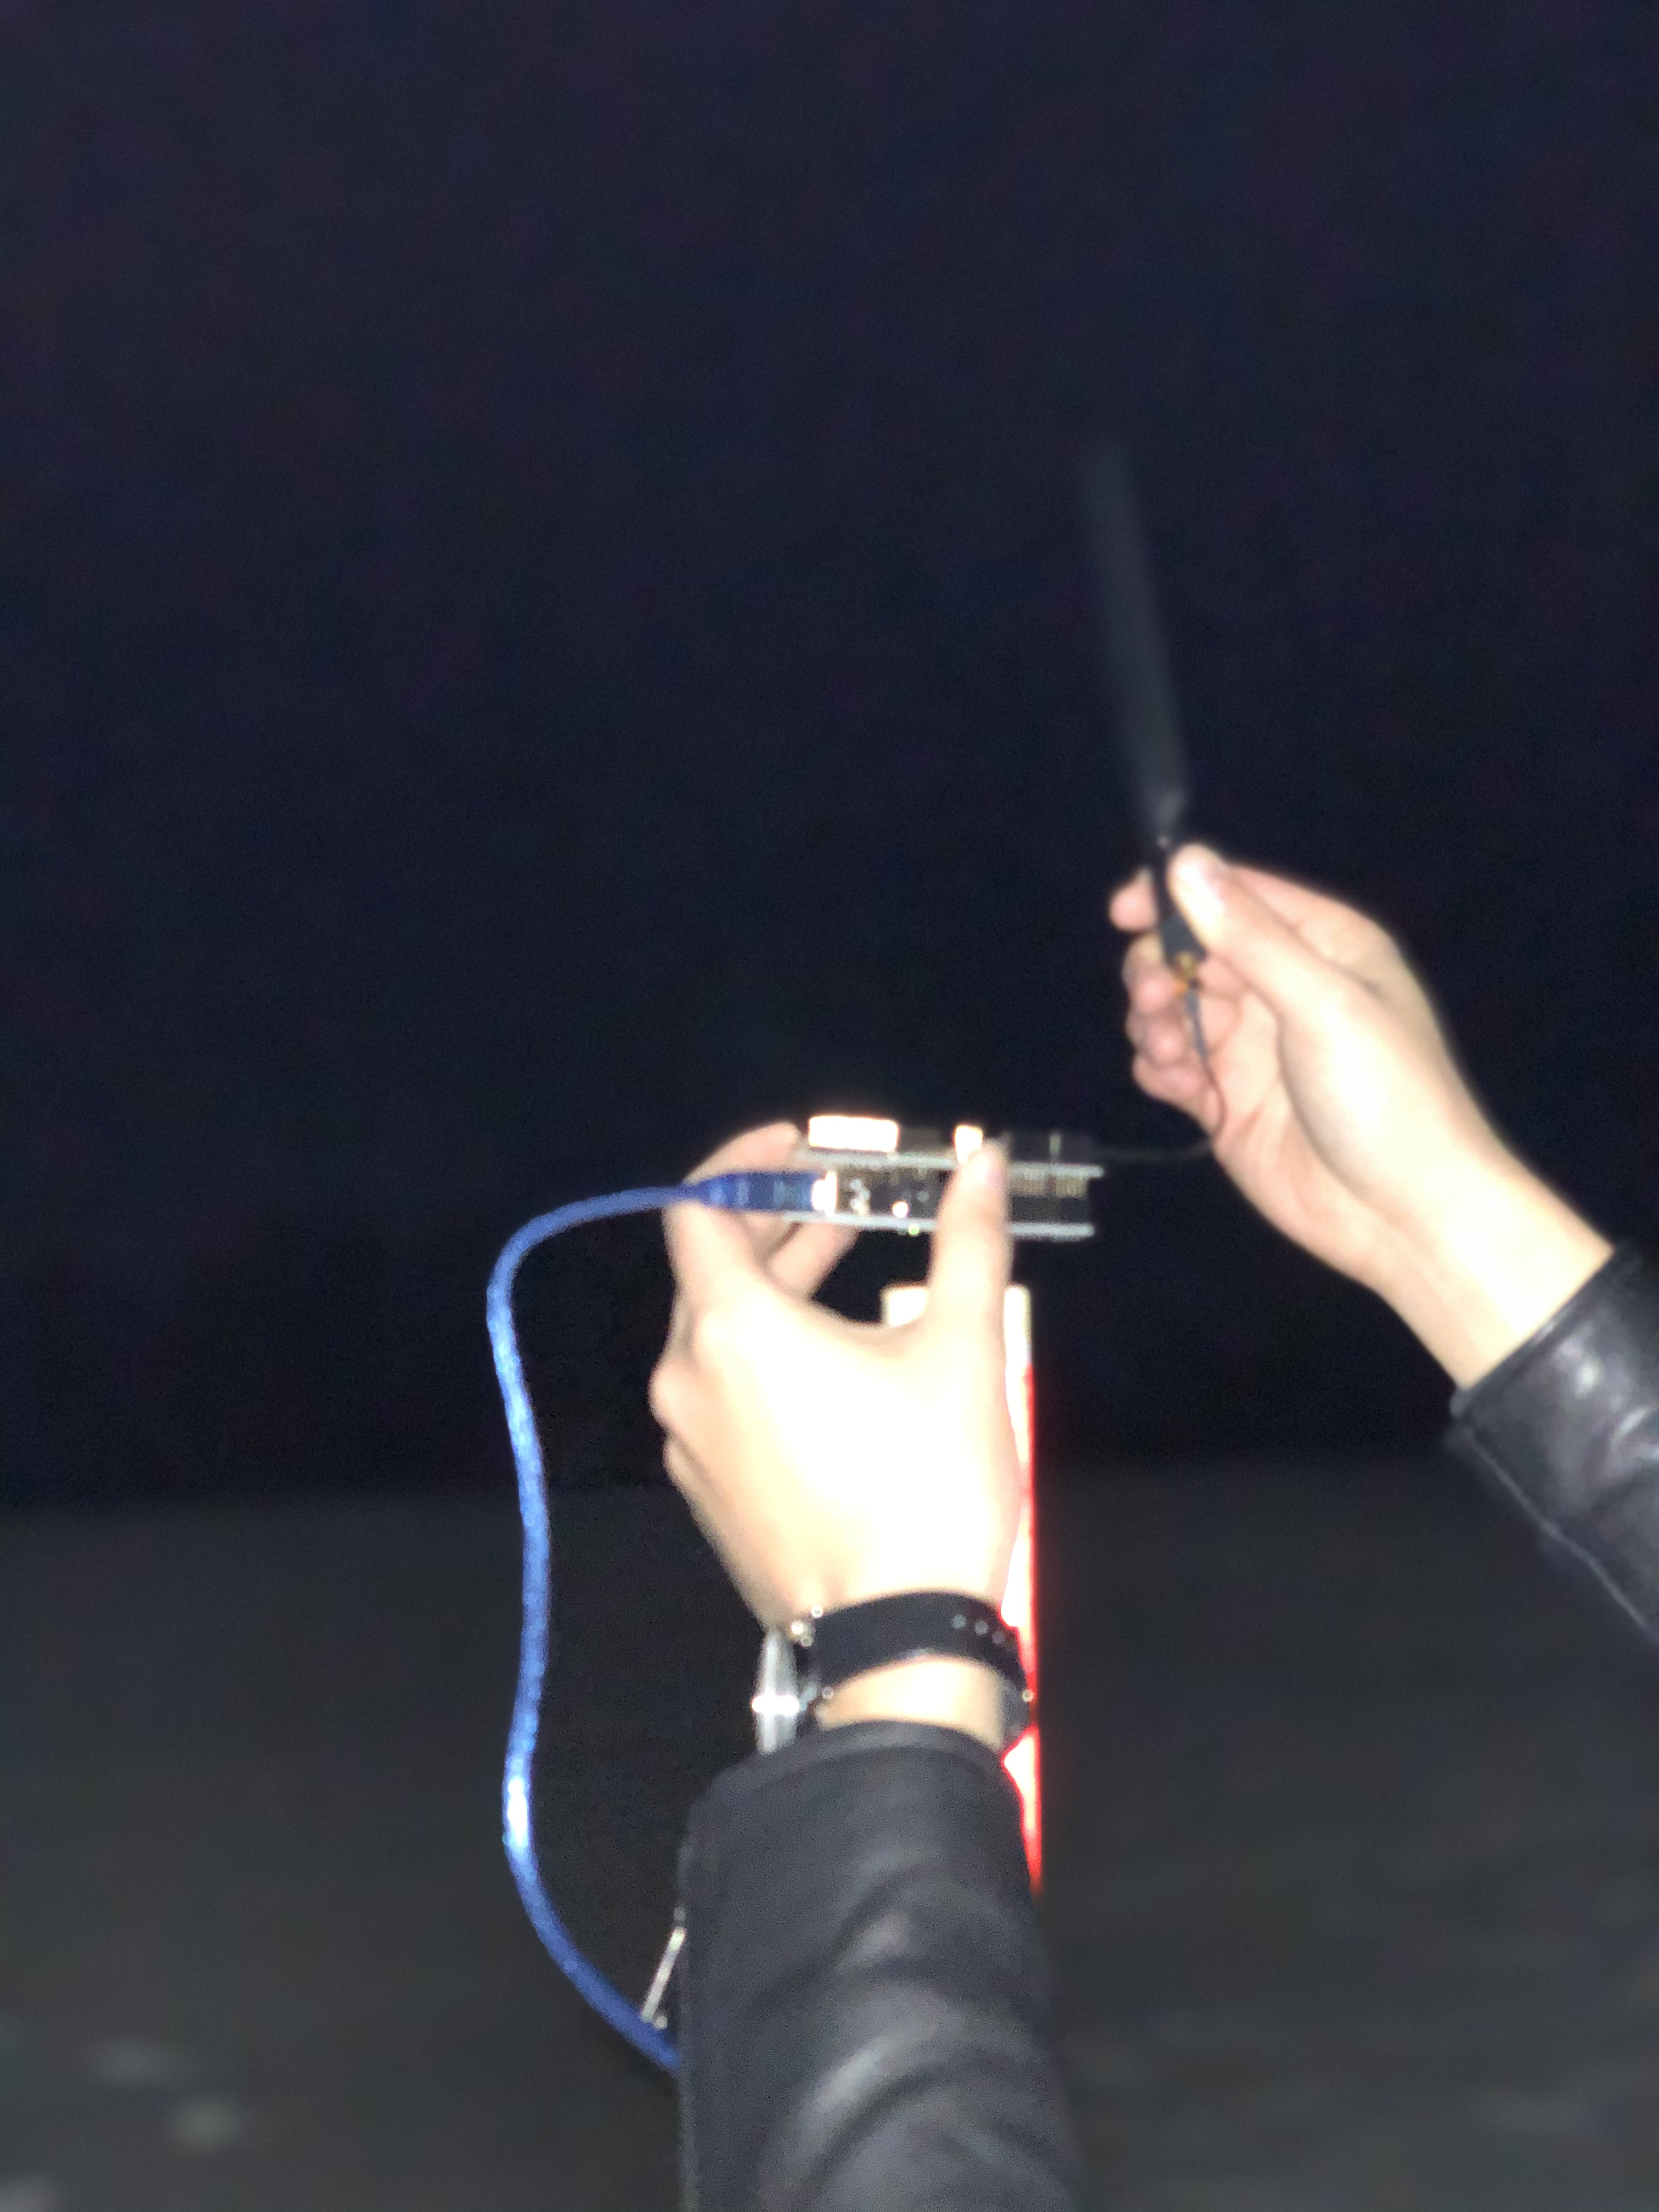
\includegraphics[width=5cm]{figures/experiment.jpg}
    \caption{実測実験の様子}
    \label{fig:experiment}
    \end{center}
\end{figure}